%%%%%%%%%%%%%%%%%%%%%%%%%%%%%%%%%%%%%%%%%%%%%%%%%%%%%%%%%%%%%%%%%%%%%%%%%%%%%
%%%
%%% File: thesis.tex, version 1.9, May 2015
%%%
%%% =============================================
%%% This file contains a template that can be used with the package
%%% cs.sty and LaTeX2e to produce a thesis that meets the requirements
%%% of the Computer Science Department from the Technical University of Cluj-Napoca
%%%%%%%%%%%%%%%%%%%%%%%%%%%%%%%%%%%%%%%%%%%%%%%%%%%%%%%%%%%%%%%%%%%%%%%%%%%%%

\documentclass[12pt,a4paper,twoside]{report}         
\usepackage{cs}              
\usepackage{times}
\usepackage{graphicx}
\usepackage{latexsym}
\usepackage{amsmath,amsbsy}
\usepackage{amssymb}
\usepackage[matrix,arrow]{xy}
\usepackage[T1]{fontenc}
\usepackage{ae,aecompl}
%\usepackage{shortcut} %definitii pentru diacritice; 
\usepackage{amstext}
\usepackage{graphics}
\usepackage[T1]{fontenc}
\usepackage{ae,aecompl}
\usepackage{algorithm}
%\usepackage{algorithmic}
\usepackage{color}
\usepackage{color}

\mastersthesis
%\diplomathesis
% \leftchapter
\centerchapter
% \rightchapter
\singlespace
% \oneandhalfspace
% \doublespace

\renewcommand{\thesisauthor}{Firstname LASTNAME}    %% Your name.
\renewcommand{\thesismonth}{June}     %% Your month of graduation.
\renewcommand{\thesisyear}{2015}      %% Your year of graduation.
\renewcommand{\thesistitle}{LICENSE THESIS TITLE} 
\renewcommand{\thesissupervisor}{scientific title Firstname LASTNAME}
\newcommand{\department}{\bf FACULTY OF AUTOMATION AND COMPUTER SCIENCE\\
COMPUTER SCIENCE DEPARTMENT}
\newcommand{\thesis}{LUCRARE DE LICEN'T'A}
\newcommand{\utcnlogo}{
\includegraphics[width=15cm]{img/tucn.jpg}}

\newcommand{\uline}[1]{\rule[0pt]{#1}{0.4pt}}
%\renewcommand{\thesisdedication}{P\u{a}rin\c{t}ilor mei}

\begin{document}
%\frontmatter
%\pagestyle{headings}

\newenvironment{definition}[1][Definition]{\begin{trivlist}
\item[\hskip \labelsep {\bfseries #1}]}{\end{trivlist}}



%\thesistitle                    %% Generate the title page.
%\authordeclarationpage                %% Generate the declaration page.

\pagenumbering{arabic}
\setcounter{page}{4}



\begin{center}
\utcnlogo

\department

\vspace{4cm}

{\bf \thesistitle} %LICENSE THESIS TITLE}

\vspace{1.5cm}

LICENSE THESIS

\vspace{6cm}

Graduate: {\bf Firstname LASTNAME} 

Supervisor: {\bf \thesissupervisor}

\vspace{3cm}
{\bf \thesisyear}
\end{center}

\thispagestyle{empty}
\newpage

\begin{center}
\utcnlogo

\department

\end{center}
\vspace{0.5cm}

%\begin{small}
\begin{tabular}{p{7cm}p{8cm}}
 %\hspace{-1cm}& APPROVED,\\
 \hspace{-1cm}DEAN, & HEAD OF DEPARTMENT,\\
\hspace{-1cm}{\bf Prof. dr. eng. Liviu MICLEA} & {\bf Prof. dr. eng. Rodica POTOLEA}\\  
\end{tabular}
 
\vspace{2cm}

\begin{center}
Graduate: {\bf \thesisauthor}

\vspace{1cm}

{\bf \thesistitle}
\end{center}

\vspace{1cm}

\begin{enumerate}
 \item {\bf Project proposal:} {\it Short description of the license thesis and initial data}
\item {\bf Project contents:} {\it (enumerate the main component parts) Presentation page, advisor's evaluation, title of chapter 1, title of chapter 2, ..., title of chapter n, bibliography, appendices.}
\item {\bf Place of documentation:} {\it Example}: Technical University of Cluj-Napoca, Computer Science Department
\item {\bf Consultants:}
\item {\bf Date of issue of the proposal:} November 1, 2014
\item {\bf Date of  delivery:} June 18, 2015 {\it (the date when the document is submitted)}
  \end{enumerate}
\vspace{1.2cm}

\hspace{6cm} Graduate: \uline{6cm} 

\vspace{0.5cm}
\hspace{6cm} Supervisor: \uline{6cm} 
%\end{small}

\thispagestyle{empty}


\newpage
$ $
%\begin{center}
%\utcnlogo

%\department
%\end{center}

\thispagestyle{empty}
\newpage

\begin{center}
\utcnlogo

\department
\end{center}

\vspace{0.5cm}

\begin{center}
{\bf
Declara\c{t}ie pe proprie r\u{a}spundere privind\\ 
autenticitatea lucr\u{a}rii de licen\c{t}\u{a}}
\end{center}
\vspace{1cm}



Subsemnatul(a) \\
\uline{14.8cm}, 
legitimat(\u{a}) cu \uline{4cm} seria \uline{3cm} nr. \uline{4cm}\\
CNP \uline{9cm}, autorul lucr\u{a}rii \uline{2.8cm}\\
\uline{16cm}\\
\uline{16cm}\\
elaborat\u{a} \^{\i}n vederea sus\c{t}inerii examenului de finalizare a studiilor de licen\c{t}\u{a} la Facultatea de Automatic\u{a} \c{s}i Calculatoare, Specializarea \uline{7cm} din cadrul Universit\u{a}\c{t}ii Tehnice din Cluj-Napoca, sesiunea \uline{4cm} a anului universitar \uline{3cm}, declar pe proprie r\u{a}spundere, c\u{a} aceast\u{a} lucrare este rezultatul propriei activit\u{a}\c{t}i intelectuale, pe baza cercet\u{a}rilor mele \c{s}i pe baza informa\c{t}iilor ob\c{t}inute din surse care au fost citate, \^{\i}n textul lucr\u{a}rii \c{s}i \^{\i}n bibliografie.

Declar, c\u{a} aceast\u{a} lucrare nu con\c{t}ine por\c{t}iuni plagiate, iar sursele bibliografice au fost folosite cu 
respectarea legisla\c{t}iei rom\^{a}ne \c{s}i a conven\c{t}iilor interna\c{t}ionale privind drepturile de autor.

Declar, de asemenea, c\u{a} aceast\u{a} lucrare nu a mai fost prezentat\u{a} \^{\i}n fa\c{t}a unei alte comisii de examen de licen\c{t}\u{a}.

\^{I}n cazul constat\u{a}rii ulterioare a unor declara\c{t}ii false, voi suporta sanc\c{t}iunile administrative, respectiv, \emph{anularea examenului de licen\c{t}\u{a}}.

\vspace{1.5cm}

Data \hspace{8cm} Nume, Prenume

\vspace{0.5cm}

\uline{3cm} \hspace{5cm} \uline{5cm}

\vspace{1cm}
\hspace{9.4cm}Semn\u{a}tura

\thispagestyle{empty}

\newpage


%\listoftables
%\listoffigures

%\clearpage 
%\newpage

%\begin{comment}
{\color{red}{\bf De citit \^{\i}nainte} (aceast\u{a} pagin\u{a} se va elimina din versiunea final\u{a})}:
\begin{enumerate}
 \item Cele trei pagini anterioare (foaie de cap\u{a}t, foaie sumar, declara\c{t}ie) se vor lista pe foi separate (nu fa\c{t}\u{a}-verso), fiind incluse \^{\i}n lucrarea listat\u{a}. 
 Foaia de sumar (a doua) necesit\u{a} semn\u{a}tura absolventului, respectiv a coordonatorului.
 Pe declara\c{t}ie se trece data c\^{a}nd se pred\u{a} lucrarea la secretarii de comisie.
 \item Pe foaia de cap\u{a}t, se va trece corect titulatura cadrului didactic \^{\i}ndrum\u{a}tor, \^{\i}n englez\u{a} (consulta\c{t}i pagina de unde a\c{t}i desc\u{a}rcat acest document pentru lista cadrelor didactice cu titulaturile lor).
 \item Documentul curent {\bf nu} a fost creat \^{\i}n MS Office. E posibil sa fie mici diferen\c{t}e de formatare. 
\item Cuprinsul \^{\i}ncepe pe pagina nou\u{a}, impar\u{a} (dac\u{a} se face listare fa\c{t}\u{a}-verso), prima pagin\u{a} din capitolul \emph{Introducere} tot a\c{s}a, fiind numerotat\u{a} cu 1. % Pentru actualizarea cuprinsului, click dreapta pe cuprins (zona cuprinsului va apare cu gri), Update field-$>$Update entire table.
\item E recomandat s\u{a} vizualiza\c{t}i acest document \c{s}i \^{\i}n timpul edit\u{a}rii lucr\u{a}rii. % după ce activaţi vizualizarea simbolurilor ascunse de formatare (apăsaţi simbolul  din Home/Paragraph).
\item Fiecare capitol \^{\i}ncepe pe pagin\u{a} nou\u{a}. % datorită simbolului ascuns Section Break (Next Page) care este deja introdus la capitolul precedent. Dacă ştergeţi din greşeală simbolul, se reintroduce (Page Layout -> Breaks).
\item Folosi\c{t}i stilurile predefinite (Headings, Figure, Table, Normal, etc.)
\item Marginile la pagini nu se modific\u{a}.
\item Respecta\c{t}i restul instruc\c{t}iunilor din fiecare capitol.
\end{enumerate}
 
%\end{comment}

\newpage

\tableofcontents
\newpage



\chapter{Introduction - Project Context}
\pagestyle{headings}

Not long time ago, big data and the need for content analysis were idealistic, intangible concepts. However, recent developments in computer performance and the growing popularity of social media has enhanced the need for novel academic approaches in this field.

The biggest challenge with processing these huge amounts of data lies in its sheer volume. This is highly problematic in many different ways:

\begin{itemize}
 \item storing and managing data is costly and sometimes needs special structuring attention
\item irregularities across data streams often indicate the need for extra transformations
\item filtering out noise and the extraction of meaningful data from thousands of entries requires specialised algorithms, architectures and platforms which are either inaccessible or difficult to use by regular users
\end{itemize}

\section{Project context}

Social media platforms these days have a strong presence in "the Cloud", which allows more and more developers to solve the problem of storage space and scalability in a relatively easy way. The high adoption of platforms like Facebook, Twitter, Instagram and many others have resulted in the generation of hundreds of thousands of online documents, text and media alike. Such a deluge of information is highly applicable for business purposes, but in is often stuck as a "diamond in the rough". An array of new and exciting job titles has also appeared, such as "Social Media Marketer", "Social Media Manager", "Social Media Expert" and so on. Not only do they represent career alternatives for a new generation, but they are also still outliers for decision support software.

\subsection{Social Media and why people care about what it says}

While the concept of Social Media is not a new one to be precise, it is clearly just starting to engulf us. The spread of Social Media alongside the spread of worldwide Internet access, the emergence of specialised applications and the recent shift to mobile online presence are objective realities. Subjectively as well, people have become more engaged to consuming, creating and sharing content online, which is evident in newspaper sales drops, app sales increase, events "going viral" within groups and even the online presence of a political critical mass. Companies offer barter possibilities for a variety of bloggers and vloggers to push products to their followers (which is not only more effective\footnote{http://www.techrepublic.com/article/election-tech-why-social-media-is-more-powerful-than-advertising/}, but also cheaper).

No wonder social media has a stake in public decisions! But for the first time in decades, people's choices are also quite open and public. Which means that some parties can get clues about society's preferences by using public data available on platforms such as Facebook, Youtube and Twitter. Consider two basic use cases, which I will emphasise throughout the course of this thesis:

\begin{itemize}
\item What does social media say about X?
\item What does social media say about X vs. Y?
\end{itemize}

where X and Y can be public people, events, brands, companies etc. 

\subsection{Data Analysis tools today}

There are a number of current platforms for data analysis, in the large sense including chart generators, format converters and importers and data visualisation plug-ins of sorts. Crossing into the realm of powerful analysis applications, most of them are complex and confusing to non-engineers, examples including Tableau\footnote{https://public.tableau.com/s/}, RapidMiner\footnote{http://rapidminer.com} and WolframAlpha\footnote{http://www.wolframalpha.com}. Figure \ref{fig:tableau} shows Tableau's interface, which may seem quite intimidating.

\begin{figure}[ht]
    \centering
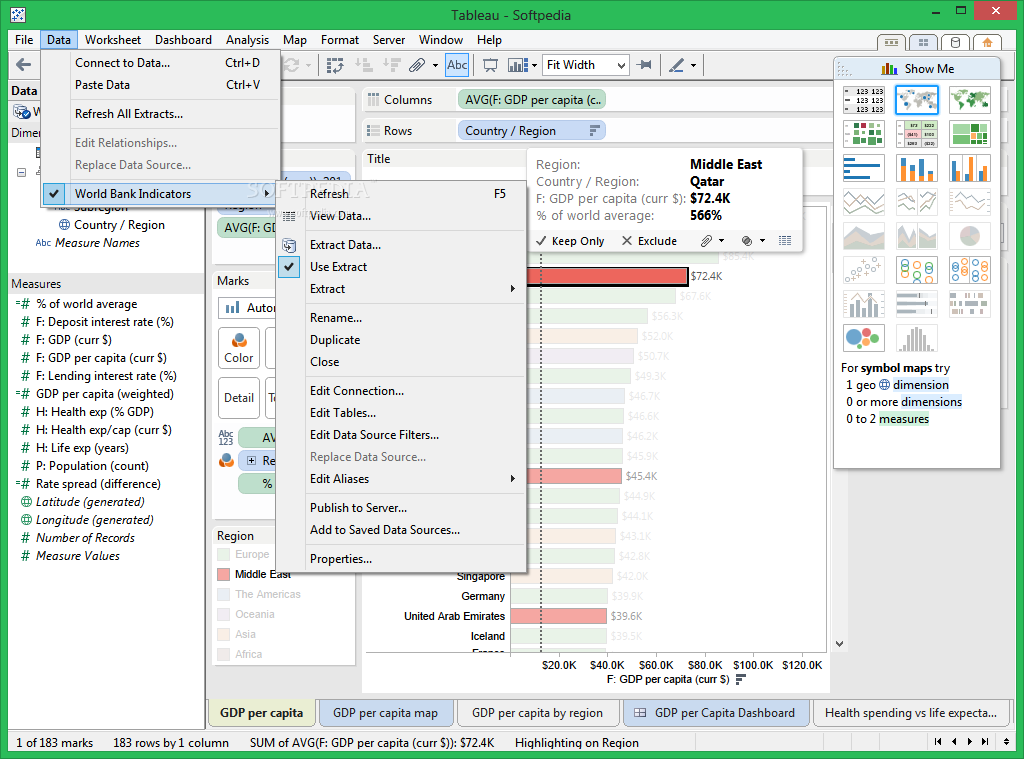
\includegraphics[width=0.8\columnwidth]{img/Tableau-Desktop_3.png}
    \caption{Tableau's interface}
    \label{fig:tableau}
\end{figure}

\subsection{Crossroads: Social Media in Business Intelligence}

The Computer Science field is very much branched nowadays in clearly-delimited subjects. But it is such a case where the large-scale processing capacities of data analytics should merge with approaches for computer-assisted business decisions. Consider that data analytics software often requires extensive training and a specialised knowledge, while most users desire only simple, straightforward functionalities for basic data analysis. One of Object Oriented Programming's fundamental principles is that of abstraction, in which end users need not (and should not) be aware of what is under the hood. Yet in data analytics, this is still the case on a 

The following Master's Thesis is the result of such an endeavour, to combine solid concepts from big data analysis, web application architecture and design, as well as enterprise software and economics for a better understanding of social media trends and opinions.

\subsection*{Thesis structure}
{\color{red} TODO
}

\chapter{Project Objectives and Specifications}
The project's purpose is to help non-expert users interested in social media analysis to get relevant and reliable information regarding specific concepts. 

\section{Web architecture}
A web architecture is preferable as a modern-day alternative to installable applications. The fast evolution of mobile devices has pushed web developers to segregate User Interfaces from Backend implementations, permitting devices to seamlessly connect to the same under the hood implementation without much development cost and overhead. Communication via REST services is crucial in this concern. Beyond user preference towards such applications, a web architecture presents even more advantages:

\begin{itemize}
\item virtually infinite space extensible with storage backends such as AWS3 or Google Cloud
\item scalability and outsourcing of time-costly services such as getting stream histories
\item database distribution over nodes
\item easily available documentation and integration throughout the development process
\end{itemize} 

Using a web framework eases development even more so and presents security advantages such as stable features, packages and quick patches in the odd case of a security breach. Plugging in services is also considered in the project's context, with handling of specific use cases done in separate managers, loosely coupled with the Model-View-Controller architecture.

\subsection{Data storage}
Since scalability and distribution are a must for a large-scale stream analysis project, data storage should be handled using a method which supports such breakdown while still remaining query-efficient. NoSQL databases are a popular choice for such implementation. The correspondence between the database storage backend and the model part of the application should also be loosely coupled, allowing for the possibility of switching between database backends if the need arises.

Big players in the field of non-relational databases are obvious possible choices: HBase, Cassandra, MongoDB, CouchDB, etc.

\section{ATHENA breakdown}
This thesis is based on the ATHENA original project, which comprises different pipeline steps in acquiring and analysing Twitter feeds:

\begin{itemize}
\item Harvesting: acquisition of collections of related Twitter statuses, by hashtag and dates (start and end).
\item Enhancement: basic analysis of a single harvest with classical unsupervised algorithms
\item Normalisation and Analysis: comparative analysis of harvests
\end{itemize}

\subsection{Twitter as data source}
For the development of this project, I chose to only implement one social media backend as data source. Twitter was the choice, since the character limit they impose is a great asset in regards of data processing: First of all, the classical data analysis pipeline deals with special cases such as documents of different lengths providing unusual skewing to the data set. Another advantage of Twitter is the prevalence of the hashtag model, which has failed to catch on with Facebook to the same degree. This means that statuses basically come out of the box already tagged for content.

Twitter is arguably the second most popular social media platform at the time, gaining on a large number of users even before the mobile device explosion, by integrating with telephone service providers to facilitate posting through SMS. Its 140 character limit makes for a good spin, which has pushed Twitter into a more textual realm than its more successful counterpart, Facebook. The platform is largely popular in the United States and especially in the entertainment domain\footnote{https://en.wikipedia.org/wiki/Twitter}, with the most popular Twitter accounts belonging to celebrities.

It notably also has a history of being the "go to" source for data analysis, after the United States' current president Barrack Obama purportedly used it in his 2008 campaign as one of the principal media outlets, choosing to have a strong Twitter presence, akin to advertisement presence of past candidates.

In short, although this approach is social platform-independent, Twitter was chosen even from the specifications step of this project for a clear start towards the data mining part.

\subsubsection{Fetching data through asynchronous jobs}
Since most social media platforms communicate with external applications via REST APIs with rate limits, the project's structure should include asynchronous modules. In this way, the user will be able to send an API-intensive job for queueing and asynchronous processing, without hindering their overall experience of using the application. This becomes apparent in the Harvesting part.

\subsection{Harvesting}
If we interpret ATHENA as a classical pipeline, then it becomes clear that the Harvesting part is the acquisition part. In order to perform analysis on data, it must first be fetched according to predefined rules and user options. Being time-intensive, these jobs must be designed asynchronously, following a FIFO model.

Figure \ref{fig:harvestpipe1} represents the conceptual model of data acquisition, starting from a collection of grouped documents (in our case they will be collections of statuses with a common hashtag). The Harvest manager handles sending asynchronous jobs via a FIFO queue towards a Consumer-type Harvesting job, represented as black box and further detailed in Figure \ref{fig:harvestpipe}. It is important to note that this pipeline is not in any way adjusted to the domain or the particular API platform; the only constraint we impose is that of periodically checking for compliance to rate limits. Social APIs usually limit requests either by number of requests or requested data size per unit of time. It is therefore a good idea to consider if any limitations alter our pipelines before starting on implementations.

\begin{figure}[ht]
    \centering
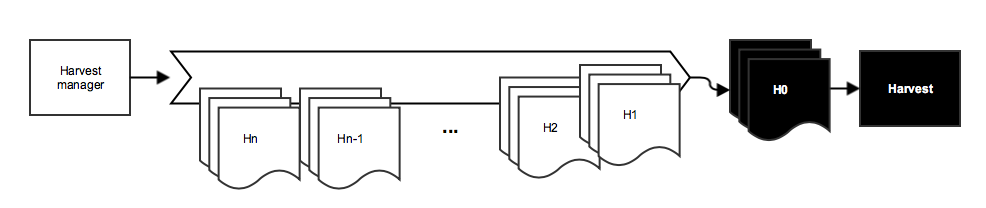
\includegraphics[width=\columnwidth]{img/harvestpipe1.png}
    \caption{Harvesting pipeline}
    \label{fig:harvestpipe1}
\end{figure}

\begin{figure}[ht]
    \centering
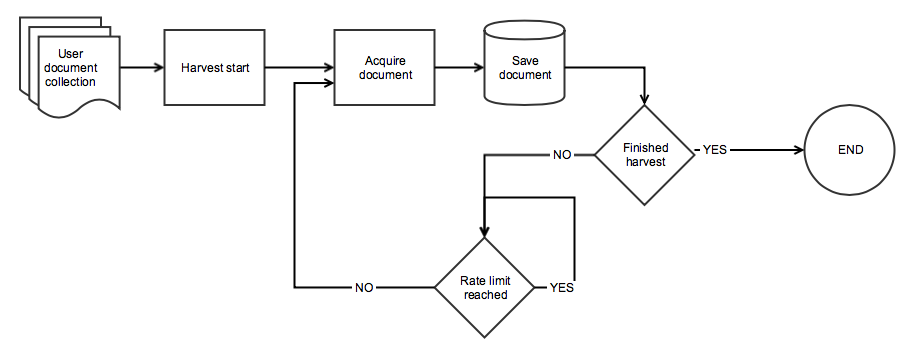
\includegraphics[width=\columnwidth]{img/harvestpipe.png}
    \caption{Harvesting job sub-pipeline}
    \label{fig:harvestpipe}
\end{figure}

\subsection{Enhancement}
As previously stated, it is not of great importance to have the data, but the goal is to obtain meaningful information from it. In this thesis I will refer to "harvests" as per the following definition:

\begin{definition}{}
A Harvest is a collection of documents related by contant, containing a token T and spanning from a start date and to an end date, which have gone through the harvesting pipeline and are stored for further anaylsis.
\end{definition}

After completing the Harvesting pipeline, resulting harvests are processed using various data extraction algorithms and presented to the user in the Enhancement step. These algorithms each have their own sub-pipelines of transformation, which will be detailed in the Analysis step.

\subsubsection{User contribution modeling}
{\color{red} TODO
}

\subsection{Normalisation and analysis}
{\color{red} TODO
}

\section{Non-functional requirements}
I am much concerned with the user's perspective in developing this application. As explained previously, one of the main objectives of this application is undoubtedly to be as simple to use as possible, to benefit non-expert users.

Firstly, I believe that a familiar and streamlined user experience should be implemented. The UI should have componenents found in most web application nowadays, in order to seem aproachable. The customisation options should also be loaded without input from the user, so that things like algorithm choices and parameters should stay hidden. Non-expert users do not know what \emph{Tfidf Vectorizer} or \emph{KMeans clustering} means, all they care about is to have some paplable results to their queries. In short, it is in the benefit of the non-expert users, which I target through this application, to have as little inputs, panels and buttons to figure out.

Besided the look and feel, users will also be interested in having a fast and reliable application. Exceptions and possible bugs should be properly filtered out and time-consuming jobs moved as per Figure \ref{fig:harvestpipe} to asynchronous jobs.

\chapter{Bibliographic research}


Bibliographic research has as an objective the establishment of the references for the project, within the project domain/thematic. While writing this chapter (in general the whole document), the author will consider the knowledge accumulated from several dedicated disciplines in the second semester, 4$^{th}$ year (Project Elaboration Methodology, etc.), and other disciplines that are relevant to the project theme.

Represents about 15\% of the paper.

Each reference must be cited within the document text, see example below (depending on the project theme, the presentation of a method/application can vary).


This section includes citations for conferences or workshop~\cite{BellucciLZ04}, journals~\cite{AntoniouSBDB07}, 
and books~\cite{russell1995artificial}. 

In paper~\cite{AntoniouSBDB07} the authors present a detection system for moving obstacles based on stereovision and ego motion estimation. 
The method is ... {\it discus the algorithms, data structures, functionality, specific aspects related to the project theme, etc.}... Discussion: {\it pros and cons}.

In chapter~\ref{ch:analysis} of~\cite{strunk}, the {\it similar-to-my-project-theme algorithm} is presented, with the following features ...


\section{Title}
\section{Other title}


\chapter{Analysis and Theoretical Foundation}
\label{ch:analysis}

Together with the next chapter takes about 60\% of the whole paper

The purpose of this chapter is to explain the operating principles of the implemented application.
Here you write about your solution from a theory standpoint - i.e. you explain it and you demonstrate its theoretical properties/value, e.g.:
\begin{itemize}
 \item used or proposed algorithms
 \item used protocols
 \item abstract models
 \item logic explanations/arguments concerning the chosen solution
 \item logic and functional structure of the application, etc.
\end{itemize}

{\color{red} YOU DO NOT write about implementation.

YOU DO NOT copy/paste info on technologies from various sources and others alike, which do not pertain to your project.
}

\section{Title}
\section{Other title}


\chapter{Detailed Design and Implementation}

Together with the previous chapter takes about 60\% of the paper.

The purpose of this chapter is to document the developed application such a way that it can be maintained and developed later. A reader should be able (from what you have written here) to identify the main functions of the application.

The chapter should contain (but not limited to):
\begin{itemize}
 \item a general application sketch/scheme,
\item a description of every component implemented, at module level,
\item class diagrams, important classes and methods from key classes.
\end{itemize}

\chapter{Testing and Validation}

About 5\% of the paper
\section{Title}
\section{Other title}

\chapter{User's manual}

In the installation description section your should detail the hardware and software resources needed for installing and running the application, and a step by step description of how your application can be deployed/installed. An administrator should be able to perform the installation/deployment based on your instructions.

In the user manual section you describe how to use the application from the point of view of a user with no inside technical information; this should be done with screen shots and a stepwize explanation of the interaction. Based on user's manual, a person should be able to use your product.

\section{Title}
\section{Other title}

\chapter{Conclusions}

About. 5\% of the whole

Here your write:
\begin{itemize}
\item a summary of your contributions/achievements,
\item a critical analysis of the achieved results,
\item a description of the possibilities of improving/further development.
\end{itemize}
\section{Title}
\section{Other title}


%\addcontentsline {toc}{chapter}{Bibliography} 
\bibliographystyle{IEEEtran} 
\bibliography{thesis}%same file name as for .bib

\appendix
\chapter{Abbreviations and shorthand}

\begin{itemize}
\item ANNIE - A Nearly-New Information Extraction System (well known set of text processing tools, used in comparison to the presented approach)
\item API - Application Programming Interface: set of entrypoints that allow the creation of an application by accessing features of another application, service etc.
\item ASCII - American Standard Code for Information Interchange: numerical represantations of characters used in computing
\item ATHENA - Approach for Tweet Harvesting, Enhancement, Normalisation and Analysis: the approach and application proof of concept presented in this thesis. It is a pipelined approach for text feature extracton from social media documents authored online
\item AWS3 - Amazon Web Simple Storage Service: a service of cloud storage provided by Amazon
\item AngularJS - popular web framework for frontend Javascript development
\item BSD - Berkeley Software Distribution License: a set of permissive free software licenses, often used in open source
\item CD - Compact Disc: a digital optical data storage format
\item CPU - Central Processing Unit: component of a computer which carries out basic instructions
\item CQL - Cassandra Query Language, a variant of the popular SQL (Structured Query Language) adapted to Cassandra non-relational databases
\item CRUD - Create, Update, Delete: Describes the functionalities of a system in reference to the actions a user can carry out on resources.
\item CSS - Cascade Style Sheet: Document which describes the appearance of a web page and not its contents.
\item CherryPy - Popular Python framework
\item CouchDB - open source non-relational database
\item DC Comics (formerly Detective Comics): American comic book publisher part of Warner Bros. Entertainment (mentioned as part of the examples section, alongside rival company Marvel)
\item DRY -  Do not Repeat Yourself: programming set of best practices which encourage code reuse without copy-pasting, thus avoiding multiple failure points
\item ERP - Enterprise Resource Planning: business process management software that allows an organization to use a system of integrated applications to manage the business and automate many back office functions
\item FIFO - First In First Out: describes the functioning of a queue, with elements being removed from the top of the queue and added at its end
\item GATE - General Architecture For Text Engineering (well known set of text processing tools, used in comparison to the presented approach)
\item GET - HTTP verb indicating fetching of a resource from the server, without any modifications
\item Git - popular version control system
\item GitHub - online project hosting using Git
\item HBase - Hadoop distributed , scalable, big data-oriented database
\item HTML - HyperText Markup Language: document describing the content of a web page, interpretable by web browsers
\item HTTP - Hypertext Transfer Protocol: application protocol for distributed, collaborative, hypermedia information systems
\item IMDB - Internet Movie DataBase: popular authoritative source for movie, TV and celebrity content (mentioned as a reliable comparison for the application results in case of movies, alongside RottenTomatoes, another popular movie review source)
\item JQuery - Javascript library which provides interactions, widgets, effects, and theming for web pages
\item JS - Javascript: is a high-level, dynamic, untyped, and interpreted programming language, usually run on the frontend side of applications and interpreted by web browsers
\item JSON - JavaScript Object Notation: lightweight data-interchange format
\item LaSIE - Large Scale Information Extraction (well known set of text processing tools, used in comparison to the presented approach)
\item LinkedIn - social media oriented toward carreer development and recruiting
\item MVC - Model/View/Controller: tripartite software architectural pattern separating internal representations of the information from their presentation to the user
\item MongoDB - non-relational database
\item NLP - Natural Language Processing
\item NLTK - Natural Language ToolKit (set of libraries and data sets for NLP)
\item NoSQL - non-SQL: database providing a mechanism for storage and retrieval of data which is modeled in ways means other than tabular relations
\item NumPy: fundamental package for scientific computing with Python
\item OAuth: open standard for authorization, commonly used as a way for Internet users to log in to third party websites using their Microsoft, Google, Facebook, Twitter, One Network etc. accounts without exposing their password
\item OSX: Apple Macintosh's Operating System
\item PHP - Hypertext Preprocessor: popular backend programming language which builds HTML files using programmatic methods
\item POST - HTTP verb indicating a modification of the resource(s) on the server
\item README.md - file which contains a short description of the application, usually placed in the codebase
\item REST - Representational State Transfer: relies on a stateless, client-server, cacheable communications protocol (usually HTTP).
\item RISC - Reduced Instruction Set Computing: CPU design strategy based on the insight that a simplified instruction set provides higher performance when combined with a microprocessor architecture capable of executing those instructions using fewer microprocessor cycles per instruction.
\item RabbitMQ: open source message broker software
\item ReactJS: popular web framework for frontend Javascript
\item RegEx - Regular Expressions: sequence of characters that define a search pattern
\item SMS - Short Message Service: text messaging service component of phone, Web, or mobile communication systems
\item SOLID - Single responsibility, open-closed, Liskov substitution, interface segregation and dependency inversion: mnemonic acronym for the "first five principles" named by Robert C. Martin in the early 2000s that stands for five basic principles of object-oriented programming
\item SQL - Structured Query Language: special-purpose language designed for managing data held in a relational database management system
\item UI - User Interface
\item URI - Uniform Resource Identifier: string of characters used to identify a resource
\item URL - Uniform Resource Locator: reference (address) to a resource on the Internet
\item UUID - Universally unique identifier: identifier standard used in software construction
\end{itemize}

\chapter{Relevant code}
\section{Fetching and saving a Harvest}
\begin{lstlisting}
def create_harvest(hashtag, start_date, end_date):
    cluster = Cluster()
    session = cluster.connect('demo')
    key = uuid.uuid1()

    session.execute(
        """
        insert into harvest (uuid, start_date, end_date, hashtag, done) values (%s, %s, %s, %s, %s)
        """,
        (key, start_date, end_date, hashtag, False)
    )

    auth = OAuthHandler(consumer_key, consumer_secret)
    auth.set_access_token(access_token, access_token_secret)
    api = tweepy.API(auth, wait_on_rate_limit=True, wait_on_rate_limit_notify=True)
    tweets = tweepy.Cursor(api.search, q='#' + hashtag, since=start_date, until=end_date, lang='en').items()

    for tweet in tweets:
        session.execute(
            """
            insert into tweet (twitterId, user, content, date, retweets, history) values (%s, %s, %s, %s, %s, %s)
            """,
            (str(tweet.id), tweet.author.screen_name.encode('utf8'), tweet.text, tweet.created_at, tweet.retweet_count, key)
        )

    session.execute(
        """
        update harvest set done=true where uuid = %s
        """,
        (key, )
    )
\end{lstlisting}

\section{Running Enhancement steps}
\subsection{Getting the document collection vocabulary}
\begin{lstlisting}
def get_vocabulary(tweet_texts):
    vectorizer = TfidfVectorizer(
        min_df=10,
        max_df=0.8,
        sublinear_tf=True,
        use_idf=True,
        max_features=25,
        token_pattern='#[a-zA-Z0-9][a-zA-Z0-9]*'
    )

    matrix = vectorizer.fit_transform(tweet_texts).toarray()
    vocabulary = vectorizer.get_feature_names()

    return vocabulary
\end{lstlisting}
\subsection{Performing clustering on the document collection}
\begin{lstlisting}

def get_clusters(tweet_texts):
    true_k = 5
    vectorizer = TfidfVectorizer(stop_words='english', min_df=10,token_pattern='#[a-zA-Z0-9][a-zA-Z0-9]*')
    X = vectorizer.fit_transform(tweet_texts)
    model = KMeans(n_clusters=true_k, init='k-means++', max_iter=100, n_init=1)
    model.fit(X)

    order_centroids = model.cluster_centers_.argsort()[:, ::-1]
    terms = vectorizer.get_feature_names()
    clusters = {}

    for i in range(true_k):
        cluster_name = 'Cluster ' + str(i+1) + ':'
        cluster = {}
        for ind in order_centroids[i, :10]:
            cluster[ind] = str(terms[ind])
        clusters[cluster_name] = cluster

    return clusters
\end{lstlisting}
\section{Normalisation by user duplication removal}
\begin{lstlisting}
def normalise(key):
    cluster = Cluster()
    session = cluster.connect('demo')
    key = uuid.UUID(key)

    res = session.execute(
        """
        select * from harvest where uuid = %s
        """,
        (key, )
    )

    for r in res:
        harvest = r

    normalised_harvest = {}

    tweets = session.execute(
        """
        select * from tweet where history = %s ALLOW FILTERING
        """,
        (key, )
    )

    no_tweets = 0

    for tweet in tweets:
        if tweet.user not in normalised_harvest.keys():
            no_tweets += 1
            normalised_harvest[tweet.user] = [tweet.twitterid, tweet.content]

    session.execute(
        """
        insert into normal (uuid, name, content) values (%s, %s, %s)
        """,
        (key, r.hashtag + ' one day normalisation', json.dumps(normalised_harvest))
    )
\end{lstlisting}

\end{document}
